\documentclass[conference]{IEEEtran}

\usepackage{amsmath}
\usepackage{amssymb}
\usepackage{graphicx}
% \usepackage{authblk}
\usepackage{float}
\usepackage{graphicx}
\usepackage[colorinlistoftodos,prependcaption,textsize=tiny]{todonotes}
\usepackage{soul}
\usepackage{algorithm}
\usepackage[noend]{algpseudocode}

%\graphicspath{ {c:/Users/mjutras/TeXworks/images/} }
\graphicspath{ {images/} }

% \author[1]{Deon Burchett, PhD}
% \author[2]{Brady Collea}
% \author[3]{Melanie Jutras}
% \author[4]{Les Servi, PhD}
% \author[5]{Randy Paffenroth, PhD}

% \affil[1,2,3,4]{The MITRE Corporation}
% \affil[5]{Worcester Polytechnic Institute}

\begin{document}

\title{ Reducing Reporting Burden of Healthcare Data Using Robust Principal Component Analysis (PCA)}
% My title isn't perfect but I think it is closer.  Let';s get it even better
%\title{Minimizing the Burden of Measuring Healthcare Data with Robust PCA}

\author{\IEEEauthorblockN{Michael Shell}
\IEEEauthorblockA{School of Electrical and\\Computer Engineering\\
Georgia Institute of Technology\\
Atlanta, Georgia 30332--0250\\
Email: http://www.michaelshell.org/contact.html}
\and
\IEEEauthorblockN{Homer Simpson}
\IEEEauthorblockA{Twentieth Century Fox\\
Springfield, USA\\
Email: homer@thesimpsons.com}
\and
\IEEEauthorblockN{James Kirk\\ and Montgomery Scott}
\IEEEauthorblockA{Starfleet Academy\\
San Francisco, California 96678--2391\\
Telephone: (800) 555--1212\\
Fax: (888) 555--1212}}

\maketitle

% FIXME: Remove before submissions!  This is just to keep track of the length as we write.
\thispagestyle{plain}
\pagestyle{plain}
\todo{Remove page numbering before submission}

\begin{abstract}
TBD TBD TBD TBD TBD TBD TBD TBD TBD TBD TBD TBD TBD TBD TBD TBD TBD TBD TBD TBD TBD
TBD TBD TBD TBD TBD TBD TBD TBD TBD TBD TBD TBD TBD TBD TBD TBD TBD TBD TBD TBD TBD
TBD TBD TBD TBD TBD TBD TBD TBD TBD TBD TBD TBD TBD TBD TBD TBD TBD TBD TBD TBD TBD
TBD TBD TBD TBD TBD TBD TBD TBD TBD TBD TBD TBD TBD TBD TBD TBD TBD TBD TBD TBD TBD
TBD TBD TBD TBD TBD TBD TBD TBD TBD TBD TBD TBD TBD TBD TBD TBD TBD TBD TBD TBD TBD
TBD TBD TBD TBD TBD TBD TBD TBD TBD TBD TBD TBD TBD TBD TBD TBD TBD TBD TBD TBD TBD
TBD TBD TBD TBD TBD TBD TBD TBD TBD TBD TBD TBD TBD TBD TBD TBD TBD TBD TBD TBD TBD
TBD TBD TBD TBD TBD TBD TBD TBD TBD TBD TBD TBD TBD TBD TBD TBD TBD TBD TBD TBD TBD
TBD TBD TBD TBD TBD TBD TBD TBD TBD TBD TBD TBD TBD TBD TBD TBD TBD TBD TBD TBD TBD
TBD TBD TBD TBD TBD TBD TBD TBD TBD TBD TBD TBD TBD TBD TBD TBD TBD TBD TBD TBD TBD
TBD TBD TBD TBD TBD TBD TBD TBD TBD TBD TBD TBD TBD TBD TBD TBD TBD TBD TBD TBD TBD
TBD TBD TBD TBD TBD TBD TBD TBD TBD TBD TBD TBD TBD TBD TBD TBD TBD TBD TBD TBD TBD
TBD TBD TBD TBD TBD TBD TBD TBD TBD TBD TBD TBD TBD TBD TBD TBD TBD TBD TBD TBD TBD
\end{abstract}

{\bf Keywords:} robust principal component analysis, anomaly
detection, health analytics, dimension reduction

\section{Introduction}

\subsection{Background}
\todo[color=yellow,]{8 Jul 2020:  This section was rewritten by LS.  I think it is in good shape but it would be nice for RP to quickly review it. }
Government agencies  mandate  metric reporting requirements to help it execute its mission.  In particular,  metrics are required for the evaluation of healthcare systems and initiatives in order to improve healthcare safety, quality and value. However, collecting and managing healthcare quality measures is expensive,  time consuming and prone to inaccuracies. These inaccuracies take two forms: Some inaccuracies are caused by the reality that attempts at precise metrics isn't always met whereas others  are wildly anomalous due to transcription errors, a misunderstanding of the precise requested metric or other business process errors.

A  proposed sets of health metrics may be unnecessarily too large and onerous because the initial analysis to design them did not properly account for redundancy of information between metrics
\todo[color=yellow,]{8 Jul  find details }Ref AcademyHealthAbstract]. Identifying the redundancy  using standard methods revolving around computing correlations between the proposed metrics is hampered because the inevitable inaccuracies in the data will give a false sense of the correlations and underlying dimensionality of the metrics.   Instead more advanced methods are required to effectively correct for imprecise inaccuracies in the data, identify and remove anomalous reported metrics, and only then examine the resulting correlations and dimensionality structure.

A promising data driven analytical approach to reduce metric reporting requirements burdens without compromising the information which can be gleaned from the data is reported in this paper. This approach is applied to real data health metrics obtained from public use files  collected over a period of one year.  However to validate the approach it was also applied  to synthetic 
  data with where ground truth is known and both small errors and anomalous errors were  intentionally inserted. 

\subsection{Contribution}
The main contribution of this research toward the problem at hand is to provide various methods which will both remove anomalies and provide a low rank approximation of the original data.  This results in significant reduction of mean squared errors (MSE) as will be shown in the results section.The impact of this research is the potential to minimize costly burden of obtaining healthcare quality data. This is especially beneficial when there is minimal information gained by the collection of the excess data. We have enhanced existing work to create fast algorithms for solving this government problem. Complete technical details of our research can be found in reference [newPaper]
\section{Analysis}

Data analysis was performed on both synthetic and real world data sets which will be described in the sections below. Analysis of synthetic data is particularly useful as we know the ground truth. Analysis of real world data sets is complicated by the fact that in many cases, we do not know ground truth.  This can make anomaly detection and dimension reduction difficult as we do not know what the outlier data points are and we also do not know the true rank of the data. 

\todo{should include bullet list}
TBD TBD TBD TBD TBD TBD TBD TBD TBD TBD TBD TBD TBD TBD TBD TBD
TBD TBD TBD TBD TBD TBD TBD TBD TBD TBD TBD TBD TBD TBD TBD TBD
TBD TBD TBD TBD TBD TBD TBD TBD TBD TBD TBD TBD TBD TBD TBD TBD
TBD TBD TBD TBD TBD TBD TBD TBD TBD TBD TBD TBD TBD TBD TBD TBD
TBD TBD TBD TBD TBD TBD TBD TBD TBD TBD TBD TBD TBD TBD TBD TBD

\begin{itemize}
\item TBD TBD TBD TBD TBD TBD TBD TBD TBD TBD TBD TBD TBD TBD TBD TBD
TBD TBD TBD TBD TBD TBD TBD TBD TBD TBD TBD TBD TBD TBD TBD TBD
\item TBD TBD TBD TBD TBD TBD TBD TBD TBD TBD TBD TBD TBD TBD TBD TBD
TBD TBD TBD TBD TBD TBD TBD TBD TBD TBD TBD TBD TBD TBD TBD TBD
\item TBD TBD TBD TBD TBD TBD TBD TBD TBD TBD TBD TBD TBD TBD TBD TBD
TBD TBD TBD TBD TBD TBD TBD TBD TBD TBD TBD TBD TBD TBD TBD TBD
\end{itemize}

\section{Background}
\subsection{Traditional PCA}
\todo{a. No anomaly handling: Matt's exhaustive search of greedy algorithm.  7 Jul (LS): Not true that the main concern about PCA is the difficulty to interpret.  We don't like PCA because it reduces the dimension of the data but it doesn't reduce the number of measurements we use.}
Traditional Principal Components Analysis (PCA) works well for dimensionality reduction, however, it is often seen as difficult to interpret.  The reason for this is that PCA produces a set of results which are linear combination of features.  This is useful for understanding the rank or underlying dimension, but does not help to select specific measures from a set of attributes. Additionally, and an important note for this research, is that PCA is extremely sensitive to outliers.  One outlier in the data can completely change the results.

In particular, consider a collection of
points $\{x_0,...,x_m\}$ with $x_i \in \mathbb{R}^n$.  Following the notation and presentation in \cite{paffenroth2018robust} we note that each point represents some object of interest, for example the $n$ measured properties of some health-care provider, the set of points $\{x_0,...,x_m\}$ would therefore
represent the collection of health-care providers that we intend to analyze.
The goal of PCA is therefore to compute a linear projection of the points $\{x_0,...,x_m\}$ into a new
set of points $\{\hat{x}_0,...,\hat{x}_m\}$ that each lay on some $k$-dimensional subspace of the original
$n$-dimensional space.  

The idea is that the subspace is chosen such that each point $x_i$ has to be moved as little as possible
to make it lay on the $k$-dimensional subspace.  If one encodes the measurement $x_i$ into a matrix
$X \in \mathbb{R}^{m \times n}$ which each $x_i$ being a row of $X$, then one can find
the low-dimensional representation $X$ by solving an optimization problem such as 

\begin{align} \label{PCAopt}
  &\min_{L} \| L-X \|_F^2 \\ \nonumber
  \text{subject to}\quad & \rho(L) \le k
\end{align}

\noindent where $\| L-X \|_F^2$ is the sum of the squares of the entries of $L-X$ (often called the Frobenius norm), $L \in \mathbb{R}^{n \times m}$ and $\rho(L)$ is the \emph{rank} of $L$
(the dimension of the subspace spanned by the rows of $L$).

The optimization problem in (\ref{PCAopt}) is often solved by way of the Singular Value
Decomposition (SVD) \cite{Eckart1936} which can be phrased as

\todo{Include SVD}

However, even more importantly for the current work, the SVD provides a natural \emph{compression} of the input data by way of


By the SVD we know that $X=U \Sigma V^T$.  If $X$ is of rank $k$ and $n<m$ we have that 
TBD TBD TBD TBD TBD TBD TBD TBD TBD TBD TBD TBD TBD TBD TBD TBD TBD TBD TBD TBD
TBD TBD TBD TBD TBD TBD TBD TBD TBD TBD TBD TBD TBD TBD TBD TBD TBD TBD TBD TBD
TBD TBD TBD TBD TBD TBD TBD TBD TBD TBD TBD TBD TBD TBD TBD TBD TBD TBD TBD TBD
TBD TBD TBD TBD TBD TBD TBD TBD TBD TBD TBD TBD TBD TBD TBD TBD TBD TBD TBD TBD
TBD TBD TBD TBD TBD TBD TBD TBD TBD TBD TBD TBD TBD TBD TBD TBD TBD TBD TBD TBD
TBD TBD TBD TBD TBD TBD TBD TBD TBD TBD TBD TBD TBD TBD TBD TBD TBD TBD TBD TBD
TBD TBD TBD TBD TBD TBD TBD TBD TBD TBD TBD TBD TBD TBD TBD TBD TBD TBD TBD TBD
TBD TBD TBD TBD TBD TBD TBD TBD TBD TBD TBD TBD TBD TBD TBD TBD TBD TBD TBD TBD
TBD TBD TBD TBD TBD TBD TBD TBD TBD TBD TBD TBD TBD TBD TBD TBD TBD TBD TBD TBD

% I AM NOT SURE WE NEED THIS LEVEL OF DETAIL BUT HERE IT IS FROM THE Jupyter NOTEBOOK.
% \begin{align}
% X 
% & = 
% \begin{bmatrix}
% U_{1:k,1:k} & U_{1:k,k+1:m} \\
% U_{k+1:n,1:k} & U_{k+1:n,k+1:m} \\
% \end{bmatrix}
% \begin{bmatrix}
% \Sigma_{1:k,1:k} & 0 \\
% 0 & \Sigma_{k+1:n,k+1:n} \\
% \end{bmatrix}
% \begin{bmatrix}
% V_{1:k,1:k} & V_{1:k,k+1:n} \\
% V_{k+1:n,1:k} & V_{k+1:n,k+1:n} \\
% \end{bmatrix} \\
% & = 
% \begin{bmatrix}
% U_{1:k,1:k} & U_{1:k,k+1:m} \\
% U_{k+1:n,1:k} & U_{k+1:n,k+1:m} \\
% \end{bmatrix}
% \begin{bmatrix}
% \Sigma_{1:k,1:k} & 0 \\
% 0 & 0 \\
% \end{bmatrix}
% \begin{bmatrix}
% V_{1:k,1:k} & V_{1:k,k+1:n} \\
% V_{k+1:n,1:k} & V_{k+1:n,k+1:n} \\
% \end{bmatrix} \\
% & = 
% \begin{bmatrix}
% U_{1:k,1:k} & 0 \\
% U_{k+1:n,1:k} & 0 \\
% \end{bmatrix}
% \begin{bmatrix}
% \Sigma_{1:k,1:k} & 0 \\
% 0 & 0 \\
% \end{bmatrix}
% \begin{bmatrix}
% V_{1:k,1:k} & V_{1:k,k+1:n} \\
% 0 & 0 \\
% \end{bmatrix} \\
% & = 
% \begin{bmatrix}
% U_{1:k,1:k} \\
% U_{k+1:n,1:k} \\
% \end{bmatrix}
% \begin{bmatrix}
% \Sigma_{1:k,1:k}
% \end{bmatrix}
% \begin{bmatrix}
% V_{1:k,1:k} & V_{1:k,k+1:n} \\
% \end{bmatrix} \\
% & = \hat{U} \hat{\Sigma} \hat{V}^T
% \end{align}

Unfortunately, in the current context, PCA has two important deficiencies.  First, while PCA effectively compresses the input measurements, each of the $k$ principal components in general depends on all of the $n$ original measurements.   As we are interested in not having to measure all $n$, but rather a subset, we note that TBD TBD TBD TBD TBD TBD TBD TBD TBD TBD TBD TBD TBD TBD TBD TBD TBD TBD TBD TBD TBD TBD TBD TBD TBD TBD TBD TBD TBD TBD TBD TBD TBD TBD TBD TBD TBD TBD TBD TBD.  Second, the data sets that we wish to analyze likely have outliers that are not actually part of the true representation of the data.  Unfortuantely, the squared error in (\ref{PCAopt}) TBD TBD TBD TBD TBD TBD TBD TBD TBD TBD TBD TBD TBD TBD TBD TBD TBD TBD TBD TBD TBD TBD TBD TBD TBD TBD TBD TBD TBD TBD TBD TBD TBD TBD TBD TBD TBD TBD TBD TBD.  Accordingly, we require a version of PCA what is robust to these types of measurement anomalies.   Fortunately, Robust Principal Component Analysis (RPCA) \cite{Candes2009,
 Candes2011, Chandrasekaran2009, Cai2010, Paffenroth2012a,Paffenroth2013b} provides precisely the type of approach that we require.   

\subsection{Sparse PCA}

As opposed to PCA, in which the principal components are generally linear combinations of all of the predictors, one can instead consider Sparse PCA \cite{htf01} in which individual predictors are chosen to reconstruct the rest.  In particular, TBD TBD TBD TBD TBD TBD TBD TBD TBD TBD TBD TBD TBD TBD TBD TBD TBD TBD TBD TBD TBD TBD TBD TBD TBD TBD TBD TBD TBD TBD TBD TBD TBD TBD TBD TBD TBD TBD TBD TBD.TBD TBD TBD TBD TBD TBD TBD TBD TBD TBD TBD TBD TBD TBD TBD TBD TBD TBD TBD TBD TBD TBD TBD TBD TBD TBD TBD TBD TBD TBD TBD TBD TBD TBD TBD TBD TBD TBD TBD TBD.TBD TBD TBD TBD TBD TBD TBD TBD TBD TBD TBD TBD TBD TBD TBD TBD TBD TBD TBD TBD TBD TBD TBD TBD TBD TBD TBD TBD TBD TBD TBD TBD TBD TBD TBD TBD TBD TBD TBD TBD.

For example, consider $S$ is a selection matrix with $S \in \{0,1\}^{n \times K}$ and every column of $S$ has precisely a single entry of $1$ and every row of $S$ has at most a single entry of $1$.

For example

$$
S = 
\begin{bmatrix}
1 & 0 & 0 \\
0 & 0 & 0 \\
0 & 1 & 0 \\
0 & 0 & 1 \\
0 & 0 & 0 \\
0 & 0 & 0 \\
\end{bmatrix}
$$

Selects the $1$-st, $3$-rd and $4$-th column of an $X$ that originally had $6$ columns.

So, in general we write 

$$X_K = X S$$

for selecting $k$ columns from $X$.

If were to estimate $X$ from $X_K$ we would need two properties.

First, our estimate $\hat{X}$ of $X$ should have the property that it agrees with $X$ on $S$, in other words there is some $Z$ such that

$$
\hat{X} = X S S^T + Z (I-S S^T) = X_K S^T + Z (I-S S^T)
$$

Second, our estimate $\hat{X}$ must lay on the subspace spanned by singular vectors of $X$.  Equivalently, we need that

$$
\hat{X} = \hat{X} V V^T.
$$

Plugging the first into the second we get

$$
X_K S^T + Z (I-S S^T) = (X_K S^T + Z (I-S S^T)) V V^T 
$$

expanding we get 

$$
X_K S^T + Z (I-S S^T) = X_K S^T V V^T + Z (I-S S^T)V V^T
$$

Collecting terms

$$
X_K (S^T - S^T V V^T) = Z ((I-S S^T)V V^T - (I-S S^T))
$$

which we can solve for $Z$ and \emph{only depends on $X_K$}.

\subsection{Robust PCA Convex Optimization Approach}
The Convex Optimization approach is based on Robust Principal Component Analysis (RPCA). In this section we closely follow the notation in \cite{Paffenroth2012a,Paffenroth2013b,paffenroth2018robust}. The RPCA approach will both remove anomalies and provide a low rank approximation of the original data. This is accomplished with a combination of a nuclear norm and a one norm which is regularized by a tuning parameter, $\lambda$ to induce sparsity. The Robust PCA formulation is as follows.

\begin{align} \label{RPCA}
  &\min_{L,S}\rho(L)+\lambda\|S\|_{0}\\ \nonumber
  \qquad \text{subject to} \quad &
                                   |X-(L+S)| = 0
\end{align}

\todo{Needs to be rewritten since it is copied from the arxiv paper}.
% FIXME Copied from arxiv paper
%%%%%%%%%%%%%%%%%%%%%%%%%%%%%%%%%%%%%%%%%%%%%%%%%%%%%%%%%%%%%%%%%%%%%%%%
\noindent where $\rho(L)$ is the rank of $L$, $\|S\|_{0}$ is the
number of non-zero entries in $S$, and $\lambda$ is a coupling
constant which controls the trade-off between the low-rank matrix $L$
and the sparse matrix $S$.  Unfortunately, as opposed to
\eqref{PCAopt}, we do not have any closed form solution to
\eqref{RPCA}.   Even worse, a n\"{a}ive, brute force
approach to the problem, where one searches over all possible
combinations of low-rank matrices $L$ and entries of $S$ corresponding
to a presupposed number of anomalies, would be NP-hard in the number
of anomalies.

However, Theorem 1.2 in \cite{Candes2011}, Theorem 2.1
\cite{Paffenroth2012a}, and many similar theorems in the extent
literature provide remarkable guarantees for recovery $L$ and $S$.
Providing details for these theorems would take us too far afield in
the current context, and the interested reader may refer to extent
literature for details \cite{Candes2009, candes09ex, Chandrasekaran2009,
  Candes2011, Paffenroth2012a, Paffenroth2013b}.
Herein we merely observe that the optimization in \eqref{npalg} is
NP-hard, but a closely related problem can be solved if some technical
conditions are met.\footnote{Classically, these conditions bound the
  rank of $L$, bound the sparsity of $S$, require that the columns of
  $L$ are \textit{incoherent} far from the standard basis, and require
  that the non-zero entries in $S$ are distributed uniformly.}

In particular, assuming such conditions are met, then, with high
probability the \emph{convex} program

\begin{align} \label{mainalg}
  &\min_{L,S}\|L\|_{*}+\lambda\|S\|_{1}\\ \nonumber
  \qquad \text{subject to} \quad &
                                   |Y-(L+S)|
                                   \preceq \epsilon
\end{align}

\noindent recovers $L$ and $S$, where
$\|L\|_{*} = \sum_{i=1}^m\sigma_{i}$ is the nuclear norm of $L$ (i.e.,
the sum of the singular values of $L$) and
$\|S\|_1:= \sum_{ij}|S_{ij}|$.  $\lambda$ is as in \eqref{npalg} and
$\epsilon$ is a set of point-wise error constraints which we used to
ameliorate the noise found in real-world data.  The reader familiar
with such algorithms will no-doubt note that $\|S\|_1$ is a convex
relaxation of $\|S\|_0$, and $\|L\|_*$ is a convex relaxation of
$\rho(L)$, and such problems can be efficiently solved
\cite{Boyd2010a, Candes2009, Candes2011, Paffenroth2012a,
  Paffenroth2013b, Halko2011}.

Note, in \eqref{mainalg}, the importance of the parameters $\lambda$
and $\epsilon$.  In particular, Theorem 1.2 in \cite{Candes2011}
proves that setting $\lambda = \frac{1}{\sqrt{\max(m,n)}}$, where
$Y \in \mathbb{R}^{m \times n}$ guarantees the \emph{recovery} of $L$
and $S$ from $Y$ (assuming the constraints mentioned previously).
% FIXME Copied from arxiv paper
%%%%%%%%%%%%%%%%%%%%%%%%%%%%%%%%%%%%%%%%%%%%%%%%%%%%%%%%%%%%%%%%%%%%%%%%

Approximation methods are used as implemented in the dimredu python package and available as open source here
\todo{What about the results from Melanie et al.?}
\footnote{The Python libraries and Jupyter notebook for generating the results in this paper can be found on bitbucker.org at ANONYMOUS.}

% \subsubsection{Robust PCA Combinatorial Approach}
% \todo[color=yellow,inline]{Ok, this is important.  We are not actually doing any Sparse PCA!?   This indicates we are just doing Robust PCA.   That does agree with my memory, now that I think about it.  This makes things easier, but I am not sure what the combinatorial approach is anymore.}
% \todo[inline]{Insert Deon's Problem Formulation here}

\section{Data: Synthetic and real-world}

\subsection{Synthetic Data}

Creation of synthetic data relies upon the following variables :
\begin{itemize}
\item $m$: total number of samples
\item $n$: total number of features 
\item $k$: number of independent features
\item $numAnoms$: number of anomalies in the data
\item $sizeAnom$: size of each anomaly
\item $noiseSize$: standard deviation of $0$-mean Gaussian noise added to each element of the matrix 
\end{itemize}

Based upon the above variable definitions, a synthetic data matrix $X$ is then created using the following steps
\begin{enumerate}
\item Initially, two matrices $U \in \mathbb{R}^{m \times k}$ and $V \in \mathbb{R}^{k \times n}$ are constructed and a low-rank matrix $L$ is constructed by setting $L = UV$.
\item An anomaly matrix $S$ of the same size as $L$ is constructed.  Each of the entries of $S$ is $0$ except for $numAnoms$ entries, selected uniformly at random, which are set to $sizeAnoms$.
\item A noise matrix $N$ of the same size as $L$ is constructed. Each of the entries of $N$ is set to a random draw from a Gaussian distribution with mean $0$ and standard deviation $noiseSize$.
\end{enumerate}
\noindent Our final synthetic $X$ matrix is the constructed as $X=L+S+N$.  In particular, this model is faithful to our health data since TBD TBD TBD TBD TBD TBD TBD TBD TBD TBD TBD TBD TBD TBD TBD TBD TBD TBD TBD TBD TBD TBD TBD TBD TBD TBD TBD TBD TBD TBD TBD TBD TBD TBD TBD TBD TBD TBD TBD TBD.TBD TBD TBD TBD TBD TBD TBD TBD TBD TBD TBD TBD TBD TBD TBD TBD TBD TBD TBD TBD TBD TBD TBD TBD TBD TBD TBD TBD TBD TBD TBD TBD TBD TBD TBD TBD TBD TBD TBD TBD.TBD TBD TBD TBD TBD TBD TBD TBD TBD TBD TBD TBD TBD TBD TBD TBD TBD TBD TBD TBD TBD TBD TBD TBD TBD TBD TBD TBD TBD TBD TBD TBD TBD TBD TBD TBD TBD TBD TBD TBD.

% \subsubsection{Add Noise}
% Some of our experiments were performed on clean synthetic data as a base, while other experiments included the addition of noise. Our method for adding noise to the data was as follows. SciPy's numpy random package was used to draw random samples from a Gaussian distribution mean centered at zero with a standard deviation equal to 0.1 times the standard deviation of the clean matrix $X$ described in previous sections. The line of python code to accomplish this task is as follows.\\\\
% $noise = np.random.normal(0, 0.1*np.std(myX), myX.shape)$
% \subsubsection{Add Anomalies}
% For the purpose of our experiments, many different input files were created with varying number of anomalies as well as anomalies that were various magnitudes. The method for adding anomalies to the data was as follows.
% \begin{itemize}
% \item Randomly select a cell in the matrix
% \item Make sure an anomaly has not already been added at this location
% \item Randomly decide if we're inserting a positive or negative anomaly
% \item Insert the anomaly of size $sizeAnom$ with the randomly generated sign at the randomly selected location
% \end{itemize}

\subsection{Real Data}

The health data set that we chose to analyze was provided by the Centers for Medicare and Medicaid Services (CMS). The public use file is available at CMS.gov and contains data related to the Shared Savings Program Accountable Care Organizations (ACO) in the year 2016. The dataset consists of 432 ACOs and makes use of 34 nationally recognized Quality Measures.  A simple boxplot visualization of the normalized dataset reveals the distributions, skewed data and outliers of the various features. It is not unusual for real world data to be noisy and impacted by outliers due to human error, but it does complicate analysis.\\

\begin{figure}[H]
    \centering
    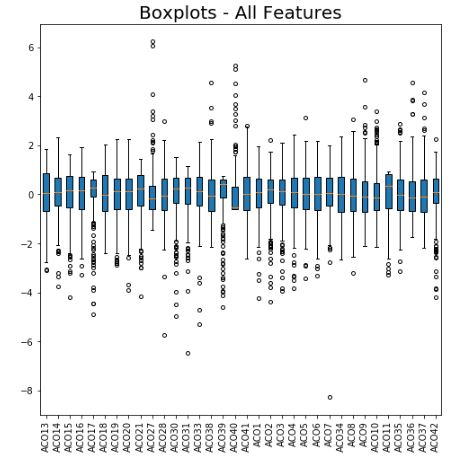
\includegraphics{BoxPlots_ALL.jpg}
    \caption{Boxplot of all features}
    \label{fig:boxall}
\end{figure}

The quality measures can be divided into distinct sub-categories. Boxplots created for each of these categories may reveal differences in the data distributions for each category of features. The GPRO features in particular appear to have greater variability and larger outliers.

\begin{enumerate}
\item GPRO - Group Practice Reporting Option Features (16 measures) : GPRO features are collected by a web interface which was designed specifically to capture ACO-reported clinical quality data.

\begin{figure}[H]
    \centering
    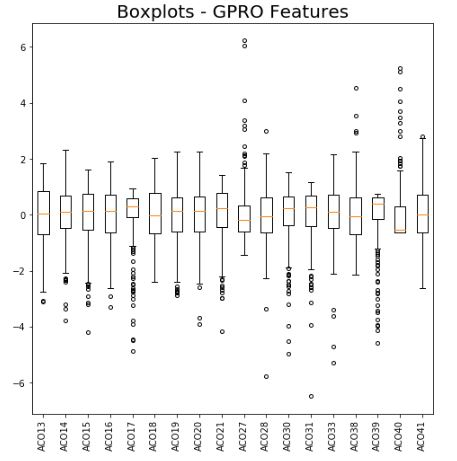
\includegraphics{BoxPlots_GPRO.jpg}
    \caption{Boxplot of GPRO features}
    \label{fig:boxgpro}
\end{figure}


\item CAHPS - Consumer Assessment of Healthcare Providers Features (10 measures) : CAHPS features are collected by a survey administered by a CMS-approved vendor selected and paid for by individual ACOs.

\begin{figure}[H]
    \centering
    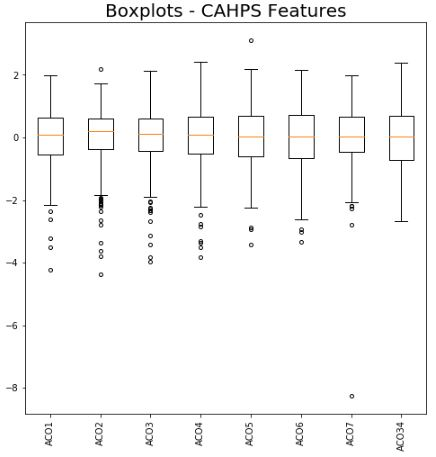
\includegraphics{BoxPlots_CAHPS.jpg}
    \caption{Boxplot of CAHPS features}
    \label{fig:boxcahps}
\end{figure}

\item EHR - Electronic Health Record Features (8 measures) : EHR features are calculated by the CMS ACO PAC based on CMS claims and administrative data extracted from the National Level Repository. 
\end{enumerate}

\begin{figure}[H]
    \centering
    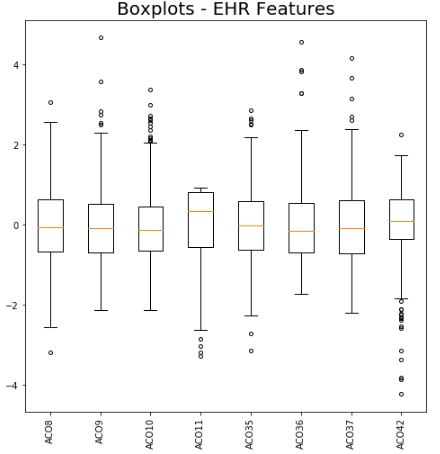
\includegraphics{BoxPlots_EHR.jpg}
    \caption{Boxplot of EHR features}
    \label{fig:boxehr}
\end{figure}



\section{Numerical Approach}

TBD TBD TBD TBD TBD TBD TBD TBD TBD TBD TBD TBD TBD TBD TBD TBD TBD TBD TBD TBD TBD TBD TBD TBD TBD TBD TBD TBD TBD TBD TBD TBD TBD TBD TBD TBD TBD TBD TBD TBD.TBD TBD TBD TBD TBD TBD TBD TBD TBD TBD TBD TBD TBD TBD TBD TBD TBD TBD TBD TBD TBD TBD TBD TBD TBD TBD TBD TBD TBD TBD TBD TBD TBD TBD TBD TBD TBD TBD TBD TBD.TBD TBD TBD TBD TBD TBD TBD TBD TBD TBD TBD TBD TBD TBD TBD TBD TBD TBD TBD TBD TBD TBD TBD TBD TBD TBD TBD TBD TBD TBD TBD TBD TBD TBD TBD TBD TBD TBD TBD TBD.

\subsubsection{Approach}

TBD TBD TBD TBD TBD TBD TBD TBD TBD TBD TBD TBD TBD TBD TBD TBD TBD TBD TBD TBD TBD TBD TBD TBD TBD TBD TBD TBD TBD TBD TBD TBD TBD TBD TBD TBD TBD TBD TBD TBD.TBD TBD TBD TBD TBD TBD TBD TBD TBD TBD TBD TBD TBD TBD TBD TBD TBD TBD TBD TBD TBD TBD TBD TBD TBD TBD TBD TBD TBD TBD TBD TBD TBD TBD TBD TBD TBD TBD TBD TBD.TBD TBD TBD TBD TBD TBD TBD TBD TBD TBD TBD TBD TBD TBD TBD TBD TBD TBD TBD TBD TBD TBD TBD TBD TBD TBD TBD TBD TBD TBD TBD TBD TBD TBD TBD TBD TBD TBD TBD TBD.

\todo{Perhaps these can be combined to make things shorter if we need space.}

In particular, the algorithm for our approach is the following when we use PCA by itself.  TBD TBD TBD TBD TBD TBD TBD TBD TBD TBD TBD TBD TBD TBD TBD TBD TBD TBD TBD TBD TBD TBD TBD TBD TBD TBD TBD TBD TBD TBD TBD TBD TBD TBD TBD TBD TBD TBD TBD TBD.TBD TBD TBD TBD TBD TBD TBD TBD TBD TBD TBD TBD TBD TBD TBD TBD TBD TBD TBD TBD TBD TBD TBD TBD TBD TBD TBD TBD TBD TBD TBD TBD

\begin{algorithm}
\caption{Euclid’s algorithm}\label{alg:euclid}
\begin{algorithmic}[1]
\Procedure{Euclid}{$a,b$}\Comment{The g.c.d. of a and b}
\State $r\gets a\bmod b$
\While{$r\not=0$}\Comment{We have the answer if r is 0}
\State $a\gets b$
\State $b\gets r$
\State $r\gets a\bmod b$
\EndWhile\label{euclidendwhile}
\State \textbf{return} $b$\Comment{The gcd is b}
\EndProcedure
\end{algorithmic}
\end{algorithm}

In particular, the algorithm for our approach is the following when we use SPCA by itself. TBD TBD TBD TBD TBD TBD TBD TBD TBD TBD TBD TBD TBD TBD TBD TBD TBD TBD TBD TBD TBD TBD TBD TBD TBD TBD TBD TBD TBD TBD TBD TBD TBD TBD TBD TBD TBD TBD TBD TBD.TBD TBD TBD TBD TBD TBD TBD TBD TBD TBD TBD TBD TBD TBD TBD TBD TBD TBD TBD TBD TBD TBD TBD TBD TBD TBD TBD TBD TBD TBD TBD TBD

\begin{algorithm}
\caption{Euclid’s algorithm}\label{alg:euclid}
\begin{algorithmic}[1]
\Procedure{Euclid}{$a,b$}\Comment{The g.c.d. of a and b}
\State $r\gets a\bmod b$
\While{$r\not=0$}\Comment{We have the answer if r is 0}
\State $a\gets b$
\State $b\gets r$
\State $r\gets a\bmod b$
\EndWhile\label{euclidendwhile}
\State \textbf{return} $b$\Comment{The gcd is b}
\EndProcedure
\end{algorithmic}
\end{algorithm}

In particular, the algorithm for our approach is the following when we use PCA by after RPCA preprocessing. TBD TBD TBD TBD TBD TBD TBD TBD TBD TBD TBD TBD TBD TBD TBD TBD TBD TBD TBD TBD TBD TBD TBD TBD TBD TBD TBD TBD TBD TBD TBD TBD TBD TBD TBD TBD TBD TBD TBD TBD.TBD TBD TBD TBD TBD TBD TBD TBD TBD TBD TBD TBD TBD TBD TBD TBD TBD TBD TBD TBD TBD TBD TBD TBD TBD TBD TBD TBD TBD TBD TBD TBD

\begin{algorithm}
\caption{Euclid’s algorithm}\label{alg:euclid}
\begin{algorithmic}[1]
\Procedure{Euclid}{$a,b$}\Comment{The g.c.d. of a and b}
\State $r\gets a\bmod b$
\While{$r\not=0$}\Comment{We have the answer if r is 0}
\State $a\gets b$
\State $b\gets r$
\State $r\gets a\bmod b$
\EndWhile\label{euclidendwhile}
\State \textbf{return} $b$\Comment{The gcd is b}
\EndProcedure
\end{algorithmic}
\end{algorithm}

In particular, the algorithm for our approach is the following when we use SPCA by after RPCA preprocessing. TBD TBD TBD TBD TBD TBD TBD TBD TBD TBD TBD TBD TBD TBD TBD TBD TBD TBD TBD TBD TBD TBD TBD TBD TBD TBD TBD TBD TBD TBD TBD TBD TBD TBD TBD TBD TBD TBD TBD TBD.TBD TBD TBD TBD TBD TBD TBD TBD TBD TBD TBD TBD TBD TBD TBD TBD TBD TBD TBD TBD TBD TBD TBD TBD TBD TBD TBD TBD TBD TBD TBD TBD

\begin{algorithm}
\caption{Euclid’s algorithm}\label{alg:euclid}
\begin{algorithmic}[1]
\Procedure{Euclid}{$a,b$}\Comment{The g.c.d. of a and b}
\State $r\gets a\bmod b$
\While{$r\not=0$}\Comment{We have the answer if r is 0}
\State $a\gets b$
\State $b\gets r$
\State $r\gets a\bmod b$
\EndWhile\label{euclidendwhile}
\State \textbf{return} $b$\Comment{The gcd is b}
\EndProcedure
\end{algorithmic}
\end{algorithm}



% \begin{enumerate}
% \item Create data with rank 6 where we know precisely the relationships between all columns
% \item Insert outliers
% \item Split matrix X into XTrain/XTest
% \item Normalize each column of the training set
% \item Set a threshold to flag values in S as outliers when running RPCA
% \item Run RPCA iteratively with different $\lambda$ values until the expected number of anomalies appear in S
% \item Generate L, S
% \item Unnormalize L to return data to original scale
% \item Compute $\alpha$ in $A\alpha = B$ in the training set for each column, resulting in 14 vectors of length 6 (one for each column), explaining the relationship between the first 6 columns and the column in question
% \item User the first 6 columns of the XTest and $\alpha$ to predict columns 7-20
% \item Compute MSE of predictions only on points which are truly not outliers
% \end{enumerate}

\section{Results}
The following results demonstrate a comparison of traditional methods and Robust Principal Components Analysis performed on synthetic data with noise and varying amounts and sizes of anomalies added.  The plots reveal that RPCA is able to detect the true rank of the data (which was created to be of rank-6), while PCA has trouble detecting the rank as it is thrown off by the noise and outliers.  Additional evidence is provided in the confusion matrix plots which show a significantly better False Positive rate using the RPCA method.

% Insert Figures for three percent anomalies size 5

\begin{figure}[H]
    \centering
    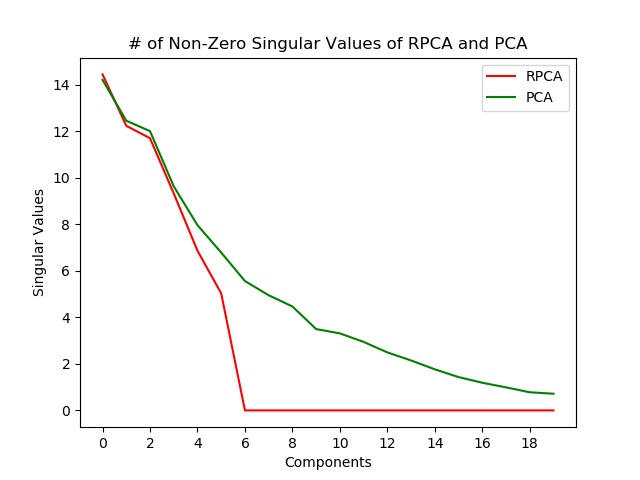
\includegraphics[width=50mm, scale=0.5]{Singular_Value_Plot_Test_120AnomSize5.jpg}
    \caption{Singular Value comparison for PCA and RPCA on synthetic data with 3 percent anomalies of size 5}
    \label{fig:singvaltrain1205}
\end{figure}

\begin{figure}[H]
    \centering
    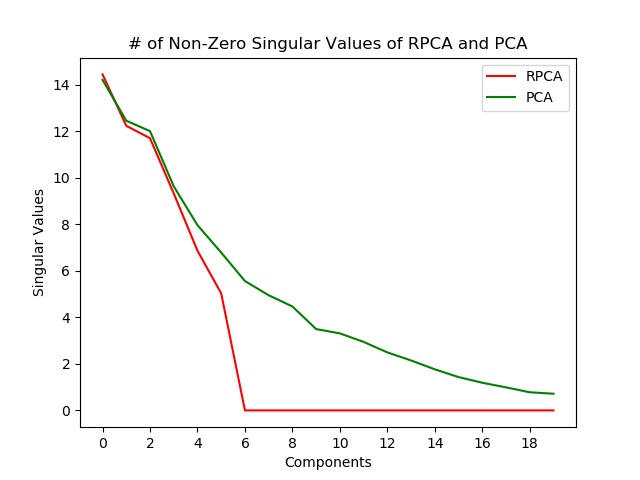
\includegraphics[width=50mm, scale=0.5]{Singular_Value_Plot_Test_120AnomSize5.jpg}
    \caption{Singular Value comparison for PCA and RPCA on synthetic data with 3 percent anomalies of size 5}
    \label{fig:singvaltrain1205}
\end{figure}

\begin{figure}[H]
\begin{minipage}[b]{0.45\linewidth}
    \centering
    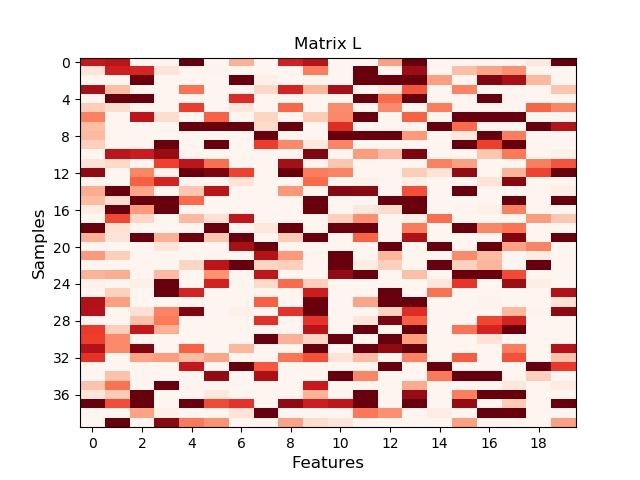
\includegraphics[width=45mm, scale=0.5]{L_120AnomSize5.jpg}
    \caption{Low-Rank Matrix resulting from RPCA on synthetic data with 3 percent anomalies of size 5}
    \label{fig:Ltrain1205}
\end{minipage}
\quad
\begin{minipage}[b]{0.45\linewidth}
    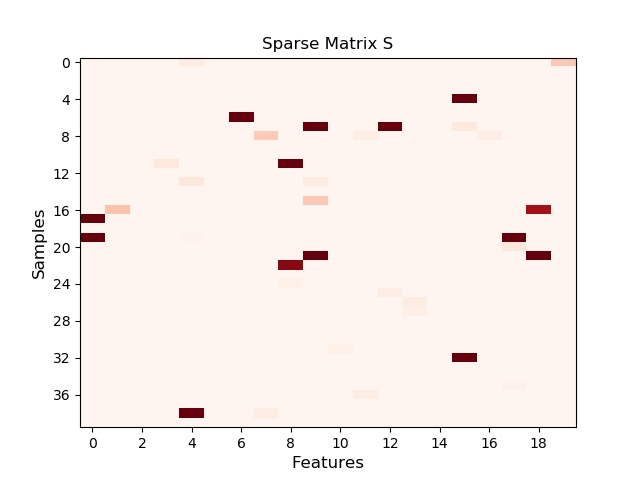
\includegraphics[width=45mm, scale=0.5]{S_120AnomSize5.jpg}
    \caption{Sparse Matrix resulting from RPCA on synthetic data with 3 percent anomalies of size 5}
    \label{fig:Strain1205}
\end{minipage}
\end{figure}

\begin{figure}[H]
\begin{minipage}[b]{0.45\linewidth}
    \centering

    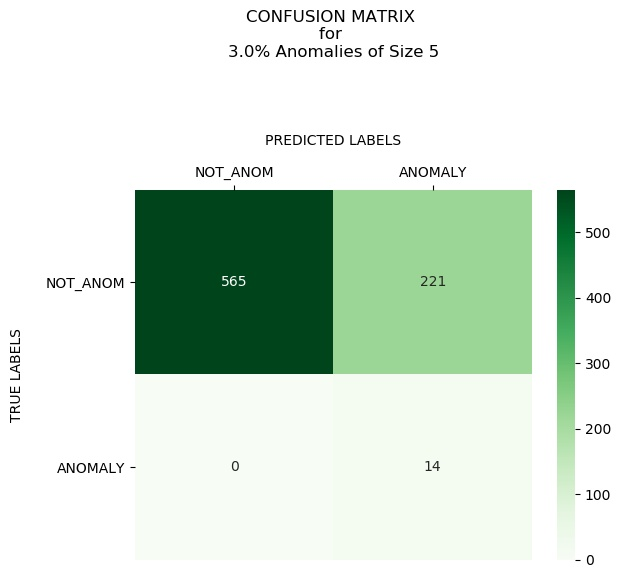
\includegraphics[width=50mm, scale=0.5]{cmPCATest_120AnomSize5.jpg}
    \caption{Confusion Matrix resulting from PCA on synthetic data with 3 percent anomalies of size 5}
    \label{fig::CMtrainPCA1205}
\end{minipage}
\quad
\begin{minipage}[b]{0.45\linewidth}
    \centering
    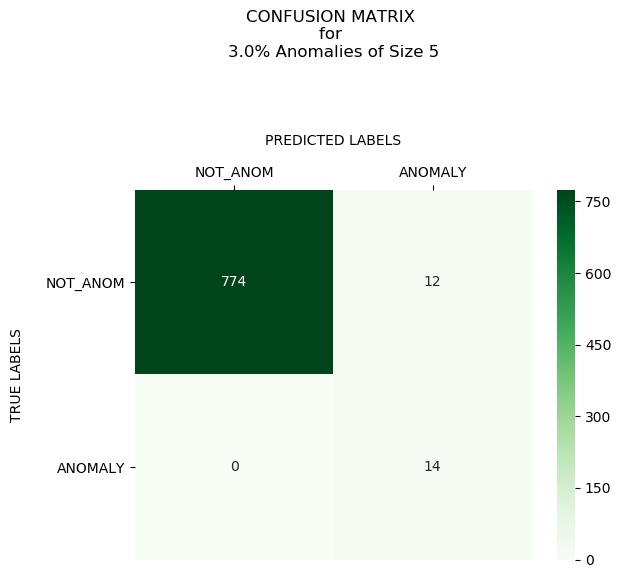
\includegraphics[width=50mm, scale=0.5]{cmRPCATest_120AnomSize5.jpg}
    \caption{Confusion Matrix resulting from RPCA on synthetic data with 3 percent anomalies of size 5}
    \label{fig::CMtrainRPCA125}
\end{minipage}
\end{figure}

% Insert Figures for three percent anomalies size 10

\begin{figure}[H]
    \centering
    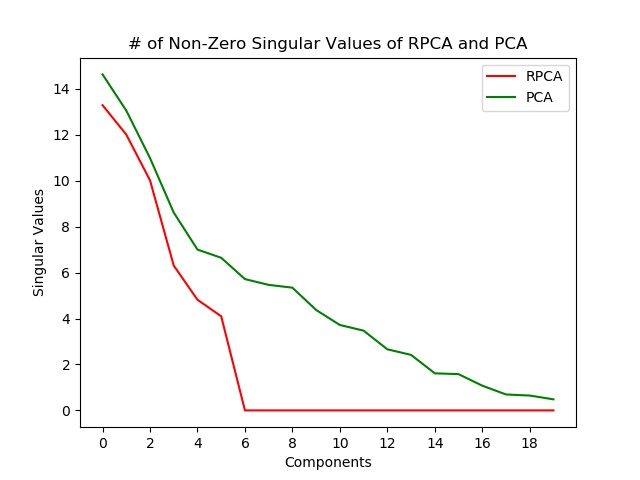
\includegraphics[width=50mm, scale=0.5]{Singular_Value_Plot_Test_120AnomSize10.jpg}
    \caption{Singular Value comparison for PCA and RPCA on synthetic data with 3 percent anomalies of size 10}
    \label{fig:singvaltrain12010}
\end{figure}
\begin{figure}[H]
\begin{minipage}[b]{0.45\linewidth}
    \centering
    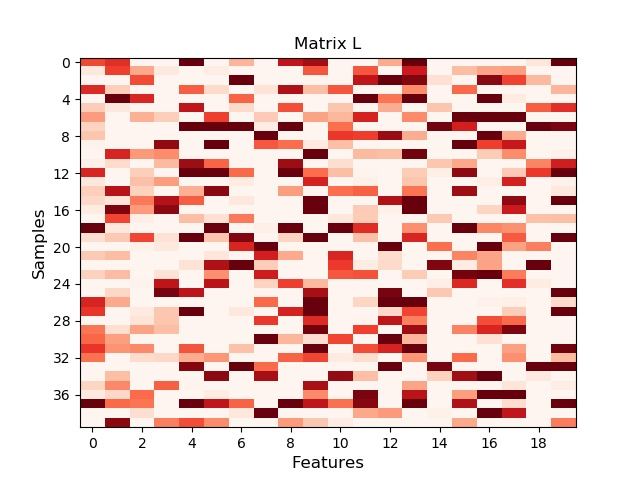
\includegraphics[width=45mm, scale=0.5]{L_120AnomSize10.jpg}
    \caption{Low-Rank Matrix resulting from RPCA on synthetic data with 3 percent anomalies of size 10}
    \label{fig:Ltrain12010}
\end{minipage}
\quad
\begin{minipage}[b]{0.45\linewidth}
    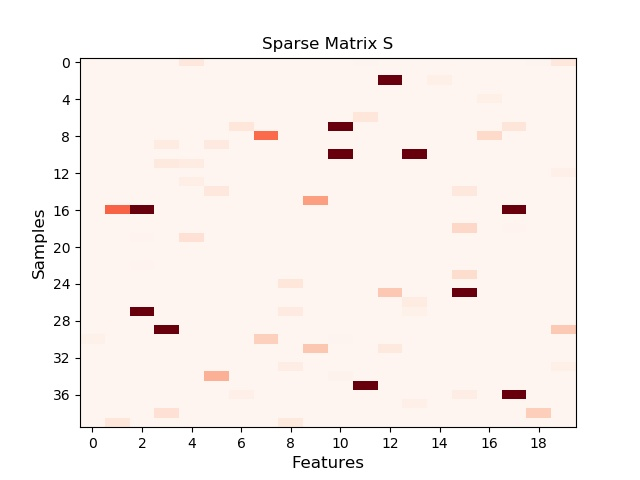
\includegraphics[width=45mm, scale=0.5]{S_120AnomSize10.jpg}
    \caption{Sparse Matrix resulting from RPCA on synthetic data with 3 percent anomalies of size 10}
    \label{fig:Strain12010}
\end{minipage}
\end{figure}

\begin{figure}[H]
\begin{minipage}[b]{0.45\linewidth}
    \centering

    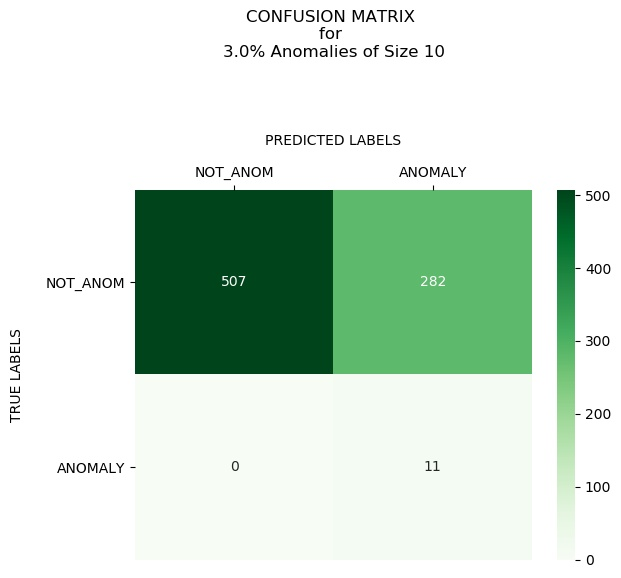
\includegraphics[width=50mm, scale=0.5]{cmPCATest_120AnomSize10.jpg}
    \caption{Confusion Matrix resulting from PCA on synthetic data with 3 percent anomalies of size 10}
    \label{fig::CMtrainPCA12010}
\end{minipage}
\quad
\begin{minipage}[b]{0.45\linewidth}
    \centering
    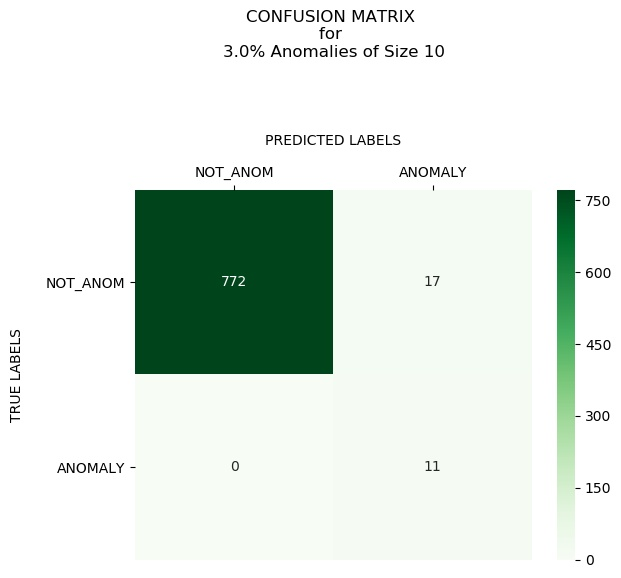
\includegraphics[width=50mm, scale=0.5]{cmRPCATest_120AnomSize10.jpg}
    \caption{Confusion Matrix resulting from RPCA on synthetic data with 3 percent anomalies of size 10}
    \label{fig::CMtrainRPCA12010}
\end{minipage}
\end{figure}

% Insert Figures for ten percent anomalies size 5

\begin{figure}[H]
    \centering
    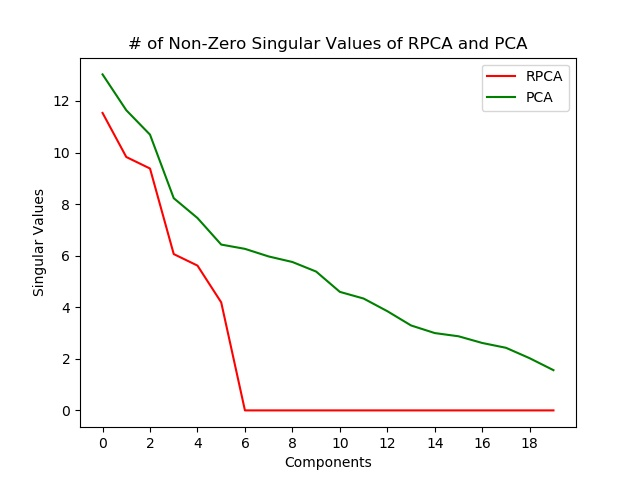
\includegraphics[width=50mm, scale=0.5]{Singular_Value_Plot_Test_400AnomSize5.jpg}
    \caption{Singular Value comparison for PCA and RPCA on synthetic data with 10 percent anomalies of size 5}
    \label{fig:singvaltrain4005}
\end{figure}
\begin{figure}[H]
\begin{minipage}[b]{0.45\linewidth}
    \centering
    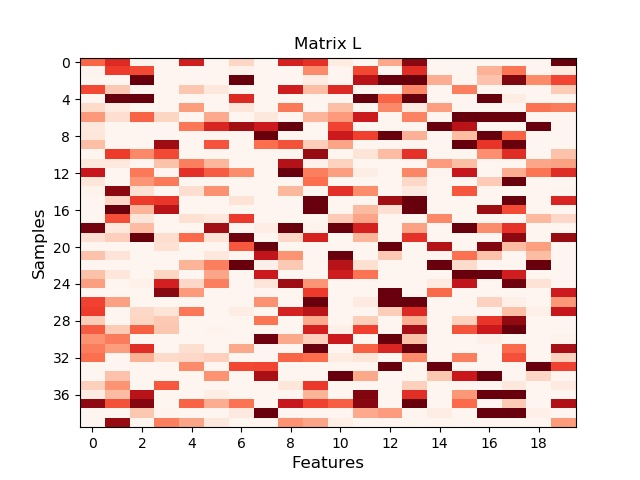
\includegraphics[width=45mm, scale=0.5]{L_400AnomSize5.jpg}
    \caption{Low-Rank Matrix resulting from RPCA on synthetic data with 10 percent anomalies of size 5}
    \label{fig:Ltrain4005}
\end{minipage}
\quad
\begin{minipage}[b]{0.45\linewidth}
    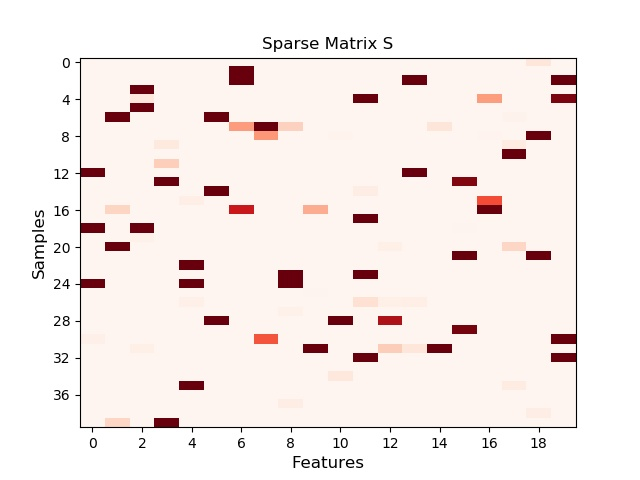
\includegraphics[width=45mm, scale=0.5]{S_400AnomSize5.jpg}
    \caption{Sparse Matrix resulting from RPCA on synthetic data with 10 percent anomalies of size 5}
    \label{fig:Strain4005}
\end{minipage}
\end{figure}

\begin{figure}[H]
\begin{minipage}[b]{0.45\linewidth}
    \centering

    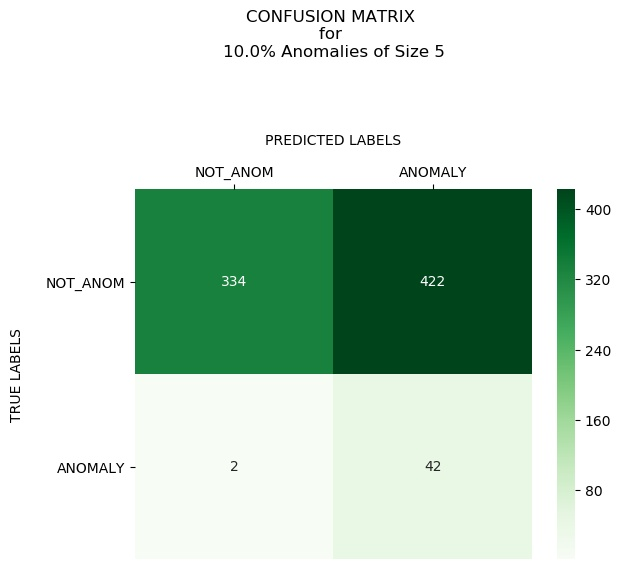
\includegraphics[width=50mm, scale=0.5]{cmPCATest_400AnomSize5.jpg}
    \caption{Confusion Matrix resulting from PCA on synthetic data with 10 percent anomalies of size 5}
    \label{fig::CMtrainPCA4005}
\end{minipage}
\quad
\begin{minipage}[b]{0.45\linewidth}
    \centering
    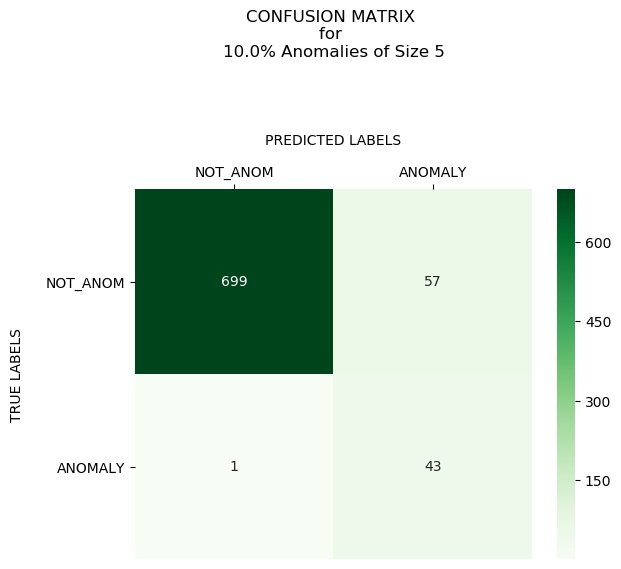
\includegraphics[width=50mm, scale=0.5]{cmRPCATest_400AnomSize5.jpg}
    \caption{Confusion Matrix resulting from RPCA on synthetic data with 10 percent anomalies of size 5}
    \label{fig::CMtrainRPCA4005}
\end{minipage}
\end{figure}

% Insert Figures for ten percent anomalies size 10

\begin{figure}[H]
    \centering
    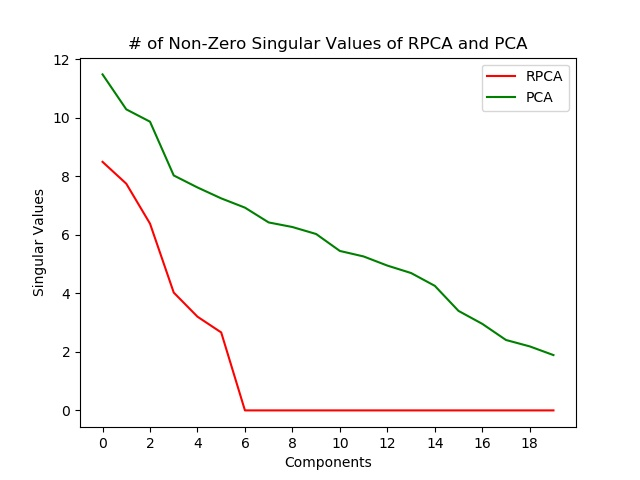
\includegraphics[width=50mm, scale=0.5]{Singular_Value_Plot_Test_400AnomSize10.jpg}
    \caption{Singular Value comparison for PCA and RPCA on synthetic data with 10 percent anomalies of size 10}
    \label{fig:singvaltrain40010}
\end{figure}
\begin{figure}[H]
\begin{minipage}[b]{0.45\linewidth}
    \centering
    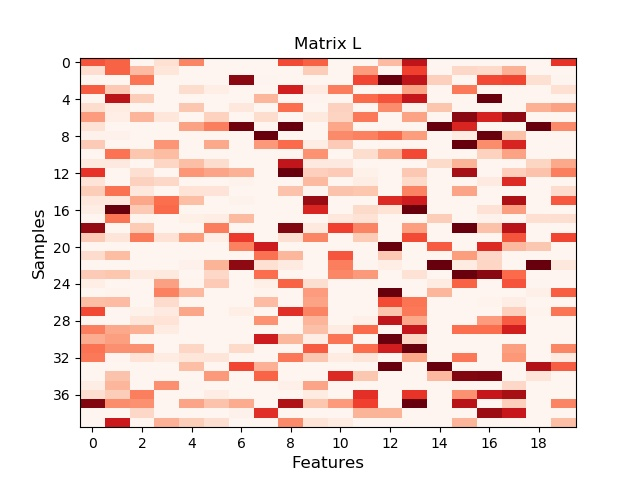
\includegraphics[width=45mm, scale=0.5]{L_400AnomSize10.jpg}
    \caption{Low-Rank Matrix resulting from RPCA on synthetic data with 10 percent anomalies of size 10}
    \label{fig:Ltrain40010}
\end{minipage}
\quad
\begin{minipage}[b]{0.45\linewidth}
    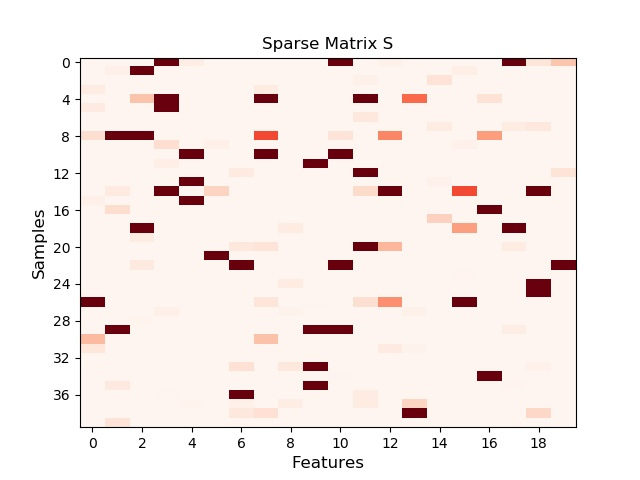
\includegraphics[width=45mm, scale=0.5]{S_400AnomSize10.jpg}
    \caption{Sparse Matrix resulting from RPCA on synthetic data with 10 percent anomalies of size 10}
    \label{fig:Strain40010}
\end{minipage}
\end{figure}

\begin{figure}[H]
\begin{minipage}[b]{0.45\linewidth}
    \centering

    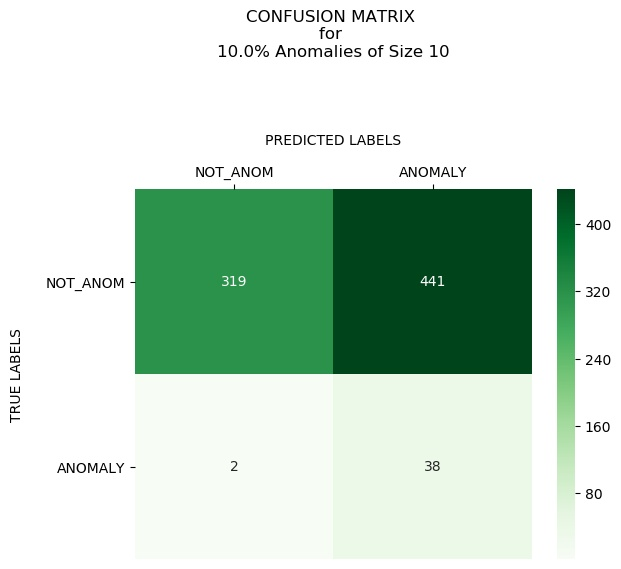
\includegraphics[width=50mm, scale=0.5]{cmPCATest_400AnomSize10.jpg}
    \caption{Confusion Matrix resulting from PCA on synthetic data with 10 percent anomalies of size 10}
    \label{fig::CMtrainPCA40010}
\end{minipage}
\quad
\begin{minipage}[b]{0.45\linewidth}
    \centering
    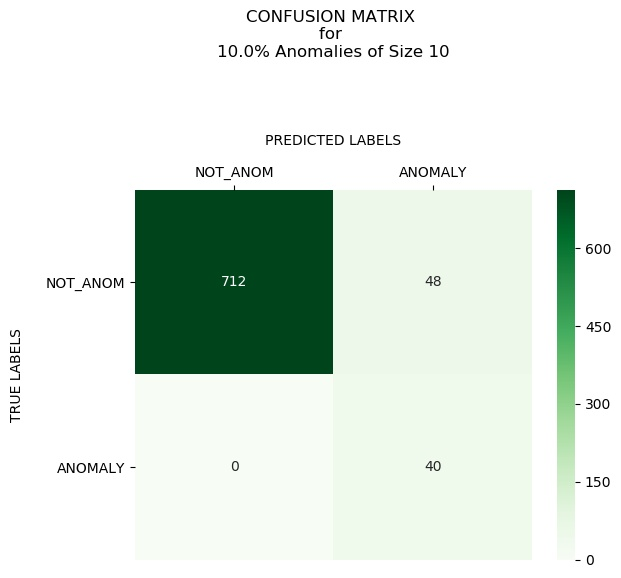
\includegraphics[width=50mm, scale=0.5]{cmRPCATest_400AnomSize10.jpg}
    \caption{Confusion Matrix resulting from RPCA on synthetic data with 10 percent anomalies of size 10}
    \label{fig::CMtrainRPCA40010}
\end{minipage}
\end{figure}

\todo[inline]{Add MSE plots of outliers against error plot data csv files}
\todo[inline]{Add results for Deon's combinatorial approach}
\todo[inline]{Add approach for real data}
\todo[inline]{Do Paffenroth insertions: add anomalies and show that we found them}
\todo[inline]{Add results for real data: What does PCA/RPCA/Gurobi find}

\section{Conclusions}

"This work suggests a new research path to explore how modern optimization methods can help complement medical and policy judgement when seeking to select health metrics from a proposed set of candidates when there is reason to expect menasurement errors and varying burden levels in the data collection process." Data analytics methods are particularly valuable for comparing various subsets of metrics when accounting for anomalies and noise due to human and measurement error. [Ref AcademyHealth Abstract]

\bibliographystyle{IEEEtran}
\bibliography{ICMLA}

\newpage
\listoftodos[Notes]
\end{document}